% Appendix B
 
\chapter{Designing Figures}

This section contains recommendations on designing effective figures. We will cover graphs as well as diagrams.

\section{Fundamental Concepts}

\subsection{Layout}

% Gestalt

% alignment
% proximity
% connectedness
% 

\subsection{Color}

\section{Diagrams}

You can use diagrams to describe concepts and their relationship, the structure of systems, interactions, and (experimental) procedures.

\subsection{Common Problems}

% infohq

% examples

\subsection{Before You Start}

Questions to ask when designing a diagram:\sidenote{Taken from the book ``Designing Science Presentations: A Visual Guide to Figures, Papers, Slides, Posters, and More'' \cite{Carter12}.}
\begin{itemize}
\item What is absolutely necessary to show?
\item What is not necessary to show?
\item What is most important and should be emphasized?
\item What is not important and should be secondary to the main message?
\item What are the relationships between individual elements?
\item Does the diagram require a precise depiction of time?
\item Does the diagram require a precise depiction of distance?
\item What symbols should be consistent throughout the diagram?
\end{itemize}


\subsection{Emphasizing Elements}

Good diagrams are self-explanatory and guide the reader's attention. Humans constantly search for patterns and deviations. Consistent use of shapes and colors indicates that the presented elements are similar (cf. Fig.~\ref{fig:emphasis}). Deviation from the norm indicate differences that need attention. Be aware of that and do not create emphasis unintentionally.

\begin{figure}[t]
\centering
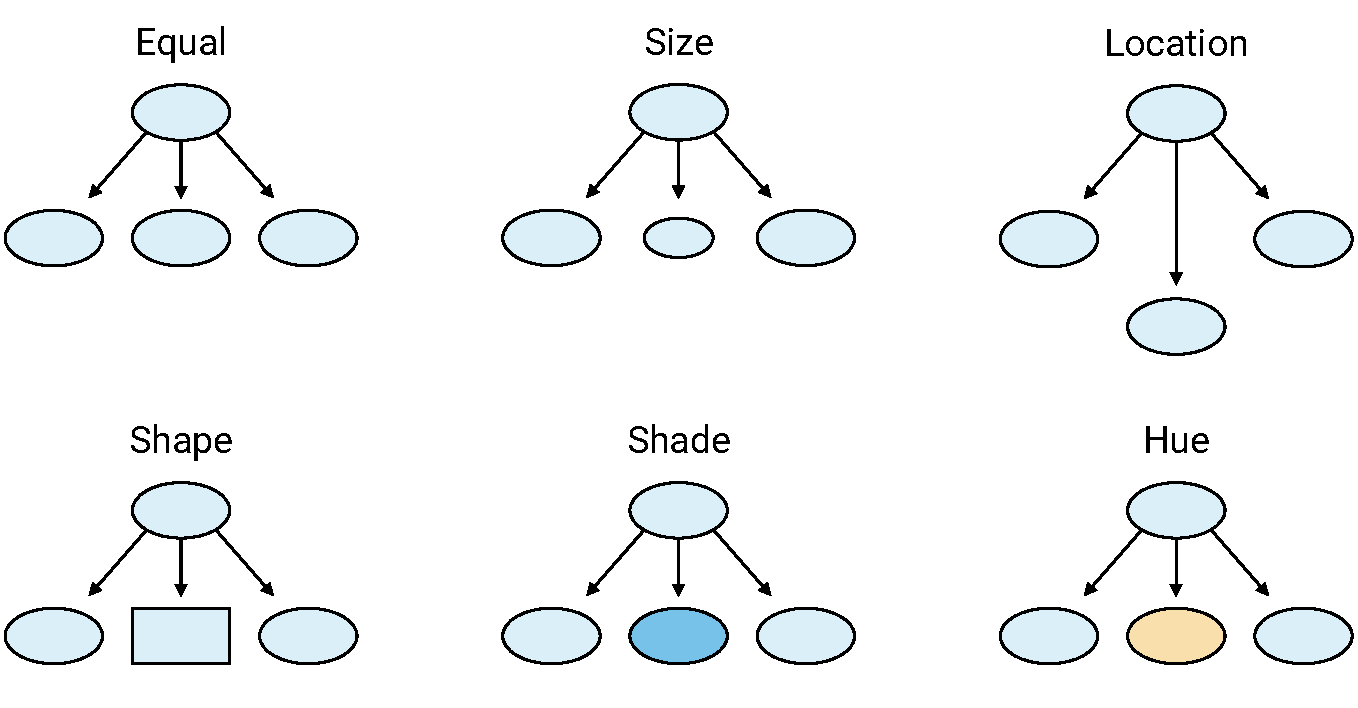
\includegraphics[width=1\textwidth]{diagram-emphasis}
\sidecaption{\label{fig:emphasis} Deviations from the norm create emphasis \cite{Carter12}.}[-4\baselineskip]
\end{figure}

Do not choose the size of elements arbitrarily. Differences translate into dominance relationships. Larger elements usually appear to control the smaller ones (cf. Fig.~\ref{fig:dominance})

\begin{figure}[t]
\centering
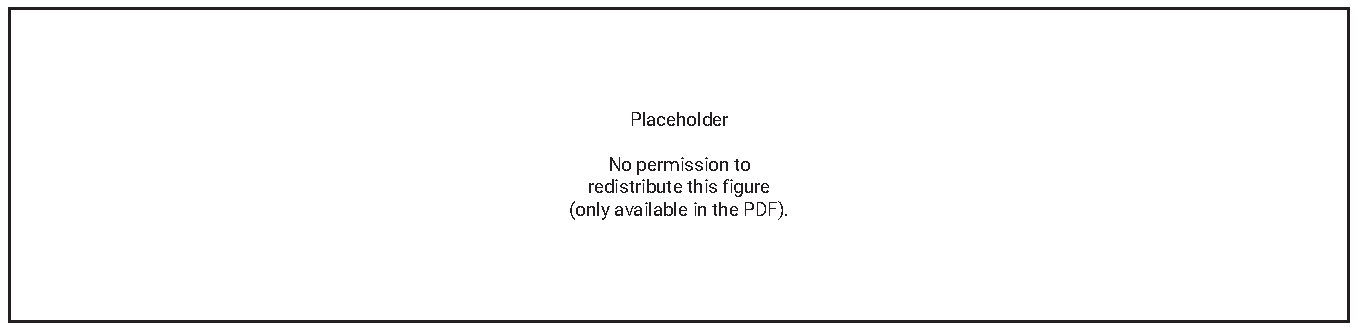
\includegraphics[width=1\textwidth]{diagram-dominance}
\sidecaption{\label{fig:dominance} Relative differences in size indicate dominance relationships \cite{Carter12}.}[-4\baselineskip]
\end{figure}


\subsection{Layout}

In the absence of strong emphasis, readers process diagrams similar to text (cf. Fig.~\ref{fig:direction}). In western cultures, readers will start in the top left corner and proceed horizontally in a zig-zag pattern. The general flow of information should be consistent with this expectation.

\begin{marginfigure}
\centering
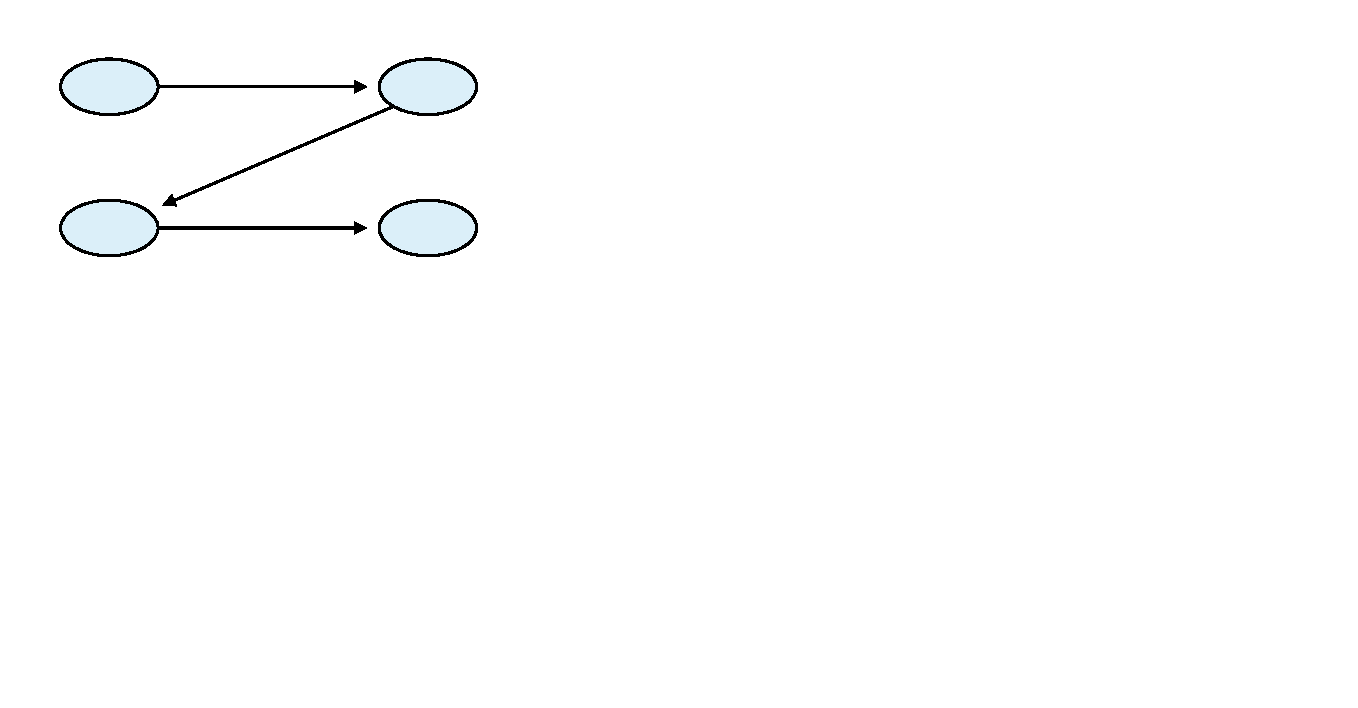
\includegraphics[width=1\textwidth]{diagram-direction}
\sidecaption{\label{fig:direction} Respect the expected flow of information in western cultures \cite{Carter12}.}[-1\baselineskip]
\end{marginfigure}


Ensure that all elements of a diagram are properly aligned. Alignment helps readers to grasp the overall structure. Proper alignment can also save you from creating additional outlines to depict (systems) boundaries – proximity and neat alignment can create strong cohesion by themselves.

Make conscious decisions about distances and dimensions (proximity, repetition). You \emph{can} use a \emph{grid} to enforce consistent distances. Note, however, that snapping every element to the grid lines, may still cause mis-alignment in some cases.\sidenote{Consider a shape that is four grid lines high. Then, a horizontal line that leaves the box cannot be aligned in the middle.} Make use of the horizontal and vertical alignment tools that space out elements equally. An advanced technique is to create a dummy box shape to measure and compare dimensions yourself.

\subsection{Labels}

Many diagrams consist of shapes and lines, annotated with text labels.

A commonplace technique is to use bold print to express some property of an element. For instance, the labels of all shapes that correspond to systems are printed in bold to differentiate these shapes from the ones that correspond to exchanged  messages. In general, we recommend to avoid this practice. Reserve bold print for emphasizing \emph{one particular element} in a diagram. Use another visual style to signify differences, such as shading, colors, or shape form. Also consider the option of giving an element no surrounding shape at all, for instance, if the notion of its \emph{boundary} is not relevant.

In any case, the labels should be as close as possible to the shapes (proximity) and exactly aligned. Whenever possible, consider moving the labels into the shapes (Fig.~\ref{labelsinside}). Inside labels reduce visual clutter and make it easier to create a well-balanced diagram that has no ragged edges.

\begin{figure}[t]
\centering
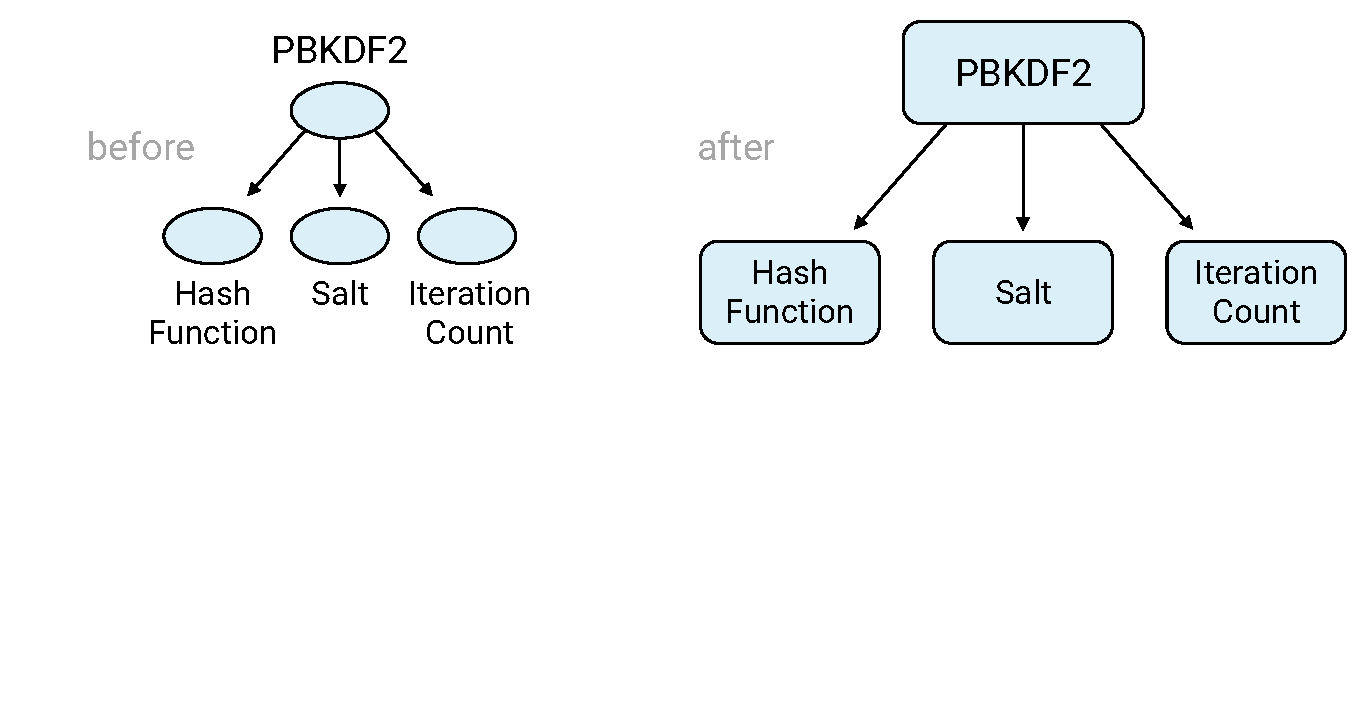
\includegraphics[width=1\textwidth]{diagram-labelsinside}
\sidecaption{\label{fig:dominance} Moving the labels inside objects reduces clutter. Note how the left-hand-side figure is centered in the left part of the figure to keep the figure balanced \cite{Carter12}.}[-6\baselineskip]
\end{figure}

Figure~\ref{fig:labelsoutside} illustrates key principles when labels are outside of a shape. First of all, keep the lines as short as possible (proximity). Consider removing the arrowheads from the lines that point into an object to avoid confusion with other arrows in the diagram. Also, avoid crossing lines. Align labels on the left-hand side of an object flush right and vice versa. Aim for consistency by making the lines parallel. Keep adequate amounts of surrounding whitespace.

\begin{marginfigure}
\centering
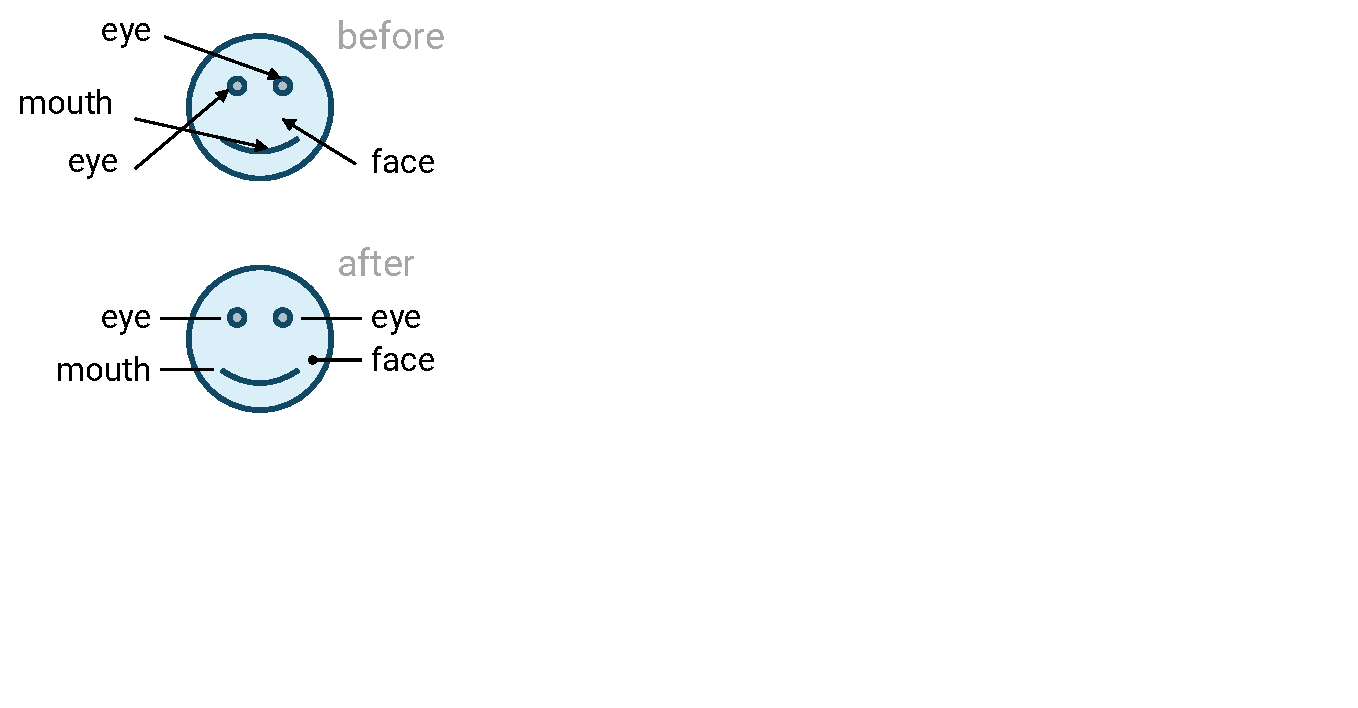
\includegraphics[width=1\textwidth]{diagram-labelsoutside}
\sidecaption{\label{fig:labelsoutside} Outside labels should not distract the reader \cite{Carter12}.}[-1\baselineskip]
\end{marginfigure}

\section{Figures}

















